\subsection{OpenStreetMap}
Um Daten von OpenStreetMap zu erhalten, kann man eine OpenStreetMap Web API ansprechen. Mapquest \cite{Mapquest} stellt eine solche OpenStreetMap API zur Verfügung. Mit dieser Schnittstelle lassen sich via HTTP GET Abfragen starten. Eine Bounding Box und die entsprechenden OpenStreetMap Tags dienen als Input. Man erhält danach alle Daten in einem einfach zu interpretierenden XML Format. Mit der gleichen Abfrage lassen sich sogar Fussgängerstreifen und Strassen zur selben Zeit herunterladen. \\

\begin{figure}[H]
	\centering
	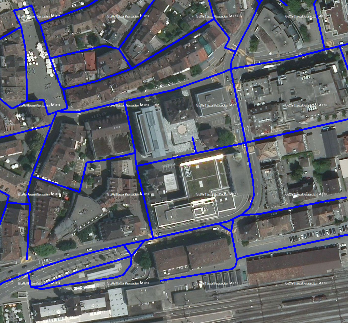
\includegraphics{images/Strassen_Rapperswil.png}
	\caption{Eingezeichnete Strassen in Rapperswil}
\end{figure}

\newpage
\subsection{Bing}
Um an die Orthofotos zu kommen, gab es zu Beginn des Projektes mehrere Lösungen:
\begin{enumerate}
	\item Offizielle Microsoft Bing REST Service
	\item Direkter Download über Bing Maps
	\item Benutzung der Orthofotos von der HSR
\end{enumerate}

Als aller erstes haben wir versucht, die Orthosfotos über den offizielle Microsoft Bing REST Service \cite{BingMapsRest} zu download. Jedoch beschränkt Microsoft den API Zugriff auf 50'000 Transaktionen pro Tag und 125'000 Transaktionen pro Jahr, was uns bei geschätzten 7 Millionen Tiles in der Schweiz nicht reichen würde.

Nachdem diesem ersten Versuch sind wir auf den direkten Download der Othosfotos umgestiegen. Wenn man mit dem Internet Browser auf Bing Maps zugreift, werden die \Gls{Tile}s mithilfe von Javascript von den Bing Servern geladen. Microsoft benutzt das Quadtree Format, um die entsprechenden Tiles anzusprechen. Mithilfe des Projekts Tiles à la Google Maps \cite{Tiles} und der dort zur Verfügung gestellten Python Library, können wir Bounding Boxen in Quadtrees umwandeln.

Die Orthofotos, welche im Besitz der HSR sind und die nur die Schweiz umfassen, wären die letzte Lösung gewesen, wenn die anderen Möglichkeiten versagt hätten.